\section{Grundlegendes zur Vererbung}

\begin{frame}[fragile]{Klassen und Instanzen}
	Eine kurze Anmerkung zum Vokabular: Um den unsäglichen Begriff \enquote{Objekt} aus diesem Kontext zunächst herauszuhalten, spreche ich von Instanzen.\\
	Eine Instanz ist ein konkretes Individuum, das nach dem Plan der Klasse erstellt wurde. Sie hat damit die Eigenschaften und Fähigkeiten, welche in der Klasse beschrieben werden.
	
	Analogie aus der Biologie: \emph{Fuchur, Olis Hund,} ist ein konkretes Individuum der Unterart Haushund. Er kann laufen (Fähigkeit) und zwar mit einer nur ihm eigenen Geschwindigkeit (Eigenschaft).
	
	\vspace{1em}
	
	Natürlich hat dieser Vergleich mit der Biologie seine Grenzen. Eine davon ist etwa, dass es dort nicht nur Unterarten gibt, sondern mehrere Ebenen von Kategorien, etwa Gattungen und Arten. In C++ hingegen gibt es nur eine Art von Kategorie: die Klasse (\verb|class|, \verb|struct|, \verb|union|).
\end{frame}

\begin{frame}[fragile]{Vererbung allgemein}
	Eine Klasse kann von anderen Klassen abgeleitet werden. Wir beschränken uns vorläufig auf die einfachste Form von Vererbung, die sogenannte \enquote{public non-virtual single inheritance}. Zur Beschreibung wollen wir zwei Klassen verwenden: \verb|CParent| und \verb|CChild|.
	
	\pause
	
	\verb|CChild| sei nun von \verb|CParent| in der genannten einfachsten Weise abgeleitet. Dann wird eine Beziehung zwischen den Klassen hergestellt.
	\begin{itemize}
		\item Eine Analogie aus der Biologie: Die Kategorie \enquote{Säugetier} ist eine Unterkategorie von \enquote{Wirbeltier}.
		\item Hier: \verb|CChild| ist eine Erweiterung von \verb|CParent|.
	\end{itemize}
	
	\pause
	
	\small
	Diese Sprechweise ist etwas ungenau, sie meint: Eine Instanz von \verb|CChild| hat \emph{alle} Eigenschaften (\enquote{data members}) und Fähigkeiten (\enquote{member functions}) einer Instanz von \verb|CParent|, sie \emph{ist auch eine Instanz der Klasse} \verb|CParent| (eine \enquote{is-a}-Beziehung).
	
	In der Biologie könnte man das ähnlich vollbringen: Olis Hund ist von der Unterart \emph{Haushund} und von der Art \emph{Wolf}.
\end{frame}

\begin{frame}[fragile]{Beispiel mit konkreten Klassen}
	\footnotesize
	\begin{columns}
		\column{0.5\textwidth}
		\lstinputlisting[language=C++, linerange=4-15]{cpp-code/CParent.h}
		
		\column{0.5\textwidth}
		\lstinputlisting[language=C++, linerange=3-13]{cpp-code/CChild.h}
	\end{columns}
	
	\pause
	\vspace{1em}
	
	Wir verwenden im Folgenden zwei »Dinge«:
	\begin{lstlisting}[lanuage=C++]
	CParent myPrObj;
	CChild  myObj;
	\end{lstlisting}
\end{frame}

\begin{frame}[fragile]{Nochmal Sprechweise}
	In unserem Beispiel ist \verb|CChild| eine \enquote{Kindklasse} von \verb|CParent|, oder andersherum: \verb|CParent| ist eine \enquote{Elterklasse}. Man spricht auch von \enquote{Basisklasse} (Elter) und \enquote{abgeleiteter Klasse} (Kind).
	
	\pause
	\vspace{1em}
	
	Statt von \enquote{Instanzen} spricht man häufig auch von \enquote{Objekten}. Der Begriff \enquote{Instanz} geht dabei mehr auf den Bezug zur Klasse ein (eine Instanz einer Klasse), während der Begriff \enquote{Objekt} tendenziell eher auf die Zusammenfassung von Eigenschaften und Fähigkeiten und die eigenständige Existenz eingeht (es existiert selbst als Objekt, nicht nur als Bündel).
	
	\pause
	\vspace{1em}
	
	Der Begriff des »Dinges« ist hiervon verschieden, da das »Ding« ein Speicherbereich ist. Es hat somit eigentlich keine member functions, diese Stecken in seinem Typen. Zudem bezeichnet in der expression \verb|int foo;| der Name \verb|foo| ein »Ding«, man würde dies in C++ aber weder eine Instanz noch ein Objekt nennen, da es keine Klasse \verb|int| gibt.
\end{frame}

\begin{frame}[fragile,b]{Die Instanz myPrObj}
	Wir wollen eine Instanz von \verb|CParent| folgendermaßen visualisieren:
	
	\vspace{2em}
	
	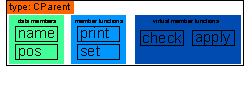
\includegraphics[width=0.5\linewidth]{images/myPrObj}
\end{frame}

\begin{frame}[fragile,b]{Zugriff auf member von myPrObj (1)}
	Zugriffe auf die einfachen (nicht-virtuellen) member functions (\enquote{Methoden}) und data members (\enquote{Eigenschaften}) funktionieren wie gehabt:
	
	\vspace{2em}
	
	\only<1>{ 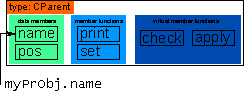
\includegraphics[width=0.5\linewidth]{images/myPrObj-name} }
	\only<2>{ 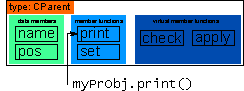
\includegraphics[width=0.5\linewidth]{images/myPrObj-print} }
\end{frame}

\begin{frame}[fragile,b]{Zugriff auf member von myPrObj (2)}
	Greifen wir über \verb|myPrObj| auf eine virtual member function zu, so bleibt alles wie gehabt:
	
	\vspace{2em}
	
	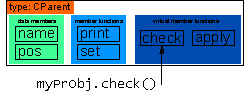
\includegraphics[width=0.5\linewidth]{images/myPrObj-check}
\end{frame}

\begin{frame}[fragile,b]{Die Instanz myObj}
	\tiny Vergessen wir ab nun die Instanz (das »Ding«) \verb|myPrObj|, sie sei hiermit entlassen.
	\normalsize
	
	\vspace{2em}
	
	Wir wollen eine Instanz von \verb|CChild| wie folgt visualisieren.
	Zu sehen ist auch das sog. \enquote{base class subobject}* von der Basisklasse CParent.\\
	\vspace{0.5em}
	\tiny
	*Das ist leider etwas verwirrend, denn ein \enquote{object} nach dem Standard haben wir bislang als »Ding« bezeichnet. Ein »Ding« enthält jedoch keine Funktionen. Ich hoffe es ist dennoch klar, dass mit dem Bild die \enquote{is-a}-Beziehung zwischen Instanzen von CChild und Instanzen von CParent zum Ausdruck gebracht werden soll.
	
	\vspace{2em}
	
	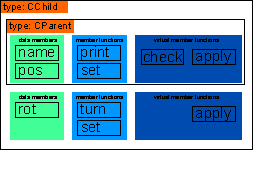
\includegraphics[width=0.5\linewidth]{images/myObj}
\end{frame}

\begin{frame}[fragile,b]{Zugriff auf member von myObj (1)}
	Zugriffe auf die einfachen (nicht-virtuellen) member functions und data members funktionieren auch hier wie gehabt:
	
	\vspace{2em}
	
	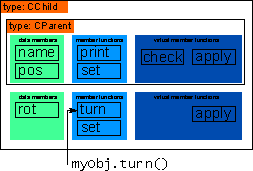
\includegraphics[width=0.5\linewidth]{images/myObj-turn}
\end{frame}

\begin{frame}[fragile,b]{Zugriff auf member von myPrObj (2) - name hiding}
	\footnotesize
	\begin{block}{name hiding (Standard 3.3.7)}
		Hat eine member function oder ein data member einer Kindklasse denselben Namen wie eine member function oder ein data member einer Basisklasse (hier: \verb|set|), so wird der Name aus der Basisklasse versteckt.
	\end{block}
	
	Etwas anschaulicher lässt es sich als \enquote{Überdecken} beschreiben: Das Element aus der Kindklasse überdeckt den Zugriff auf das Element der Basisklasse:
	
	\vspace{0.75em}
	
	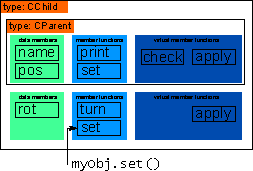
\includegraphics[width=0.5\linewidth]{images/myObj-hidingSet}
\end{frame}

\begin{frame}[fragile,b]{Zugriff auf member von myPrObj (3) - qualified-id}
	Detail (wird wirklich wirklich rar verwendet):\\
	Man kann dennoch auf das Element aus der Basisklasse zugreifen, und zwar mittels einer sog. qualified-id:
	
	\vspace{2em}
	
	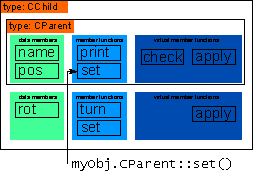
\includegraphics[width=0.5\linewidth]{images/myObj-qualifiedSet}
\end{frame}

\begin{frame}[fragile,b]{Zugriff auf member von myObj (4)}
	Zugriffe auf virtual member functions funktionieren über \verb|myObj| effektiv genauso wie Zugriffe auf normale Funktionen, allerdings ist der Mechanismus nicht das name hiding (später mehr).
	
	\vspace{2em}
	
	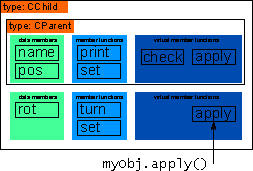
\includegraphics[width=0.5\linewidth]{images/myObj-apply}
\end{frame}

\begin{frame}[fragile,b]{Pointer und Instanzen}
	Wir können freilich einen Pointer auf \verb|myObj| anlegen: \verb|CChild* pMyObj = &myObj;|
	
	\pause
	\vspace{1em}
	
	\verb|myObj| enthält jedoch \emph{zudem} ein subobject von der Klasse \verb|CParent|. Dieses subobject hat als »Ding« ebenfalls eine Adresse, man erhält sie durch einen \enquote{implicit type cast} (Standard, 4.10:3): \verb|CParent* pMySubObj = &myObj;| (oder auch \verb|pMySubObj = pMyObj;|)
	
	\vspace{2em}
	
	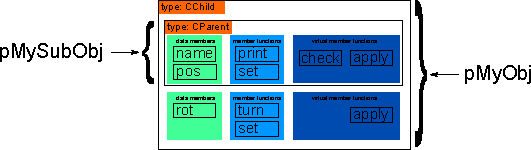
\includegraphics[width=0.75\linewidth]{images/pointers}
\end{frame}

\begin{frame}[fragile]{static type}
	\begin{block}{static type (Standard, 1.3.11)}
		Der Typ (eines »Dings« oder einer expression), so wie der Compiler ihn sieht. D.h. ohne Effekte zu berücksichtigen, die zur Laufzeit auftreten.
	\end{block}
	
	\vspace{2em}
	
	Beispiel:
	\begin{tabular}{r|l}
		\verb|int i;|	&	\verb|i| hat den static type \verb|int|	\\
		\verb|int* pi;|	&	\verb|pi| hat den static type \verb|int*|	\\
		\verb|*pi|	&	hat den static type \verb|int|	\\
		\verb|*pMySubObj|	&	hat den static type \verb|CParent|	\\
	\end{tabular}
\end{frame}

\begin{frame}[fragile]{dynamic type}
	\begin{block}{dynamic type (Standard, 1.3.3)}
		blabla lvalue blabla (unmittelbar unverständlich)
	\end{block}
	
	\vspace{2em}
	
	Beispiel:
	\begin{tabular}{r|l}
		\verb|int i;|	& \verb|i| hat den dynamic type \verb|int|	\\
		\verb|int* pi;|	& \verb|pi| hat den dynamic type \verb|int*|	\\
		\verb|*pi|	&	hat den dynamic type \verb|int|	\\
		\verb|*pMySubObj|	&	hat den dynamic type \verb|CChild|	\\
	\end{tabular}
	
	\vspace{1em}
	
	Der dynamic type ist der Typ des meist-abgeleiteten (ableiten $\implies$ Vererbung) »Dings«, auf dessen subobject ein Pointer verweist. In unserer Visualisierung entspricht dies dem Typ der übergeordnetsten Instanz.
\end{frame}

\begin{frame}[fragile,b]{Zugriff mittels pMySubObj (1)}
	Nutzt man \verb|pMySubObj|, um auf data members oder \emph{non-virtual} member functions zuzugreifen, wird der static type verwendet. Somit ist das übergeordnete des subobjects sozusagen unsichtbar. Dementsprechend wird beim Zugriff über \verb|pMySubObj| die zweite Deklaration von \verb|set| \enquote{nicht gesehen}.
	
	\vspace{2em}
	
	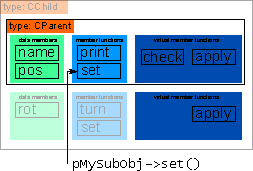
\includegraphics[width=0.5\linewidth]{images/pMySubObj-set}
\end{frame}


\section{Virtuelle Methoden}

\begin{frame}[fragile]{Overriding}
	\begin{block}{Überschreiben (Standard, 10.3:2)}
		In einer Klasse \verb|CParent| sei eine virtual member function \verb|apply| deklariert. Eine Klasse \verb|CChild| erbe direkt oder indirekt von \verb|CParent|. Wenn nun in \verb|CChild| eine Funktion mit \emph{demselben Namen und derselben Parameter-Liste} wie \verb|CParent::apply| deklariert ist, so ist \verb|CChild::apply| ebenfalls virtual (egal, ob sie so explizit deklariert wurde oder nicht) und sie \emph{überschreibt} \verb|CParent::apply|.
		Der Einfachheit halber sagt man, dass Definition der virtual member function in der Elterklasse ebenfalls eine Überschreibung ist, wenn sie nicht als pure virtual member function angelegt wurde (\emph{pure}: später).
	\end{block}
	
	\vspace{1em}
	
	Beachte: Überschreiben ist etwas Anderes als verdecken (name hiding)!
\end{frame}

\begin{frame}[fragile]{Das Aufrufen virtueller Funktionen (1)}
	\begin{block}{calling a virtual function (Standard, 5.2.2:1)}
		Wird eine virtual function aufgerufen, wird der dynamic type des »Dings« herangezogen. Es wird dann ausgehend vom dynamic type in der Vererbungshierarchie in Richtung der Elter-Klassen nach einer Überschreibung der Funktion gesucht und der erste Treffer verwendet.
	\end{block}
	
	\pause
	\vspace{1em}
	
	Normalerweise (bei nicht-virtuellen Funktionen) wird vom static type ausgegangen, daher ruft \verb|pMySubObj->set();| auch \verb|CParent::set| auf.
	\vspace{0.5em}
	Bei virtual function calls hingegen wird vom \emph{dynamic type} ausgegangen. Da der dynamic type von \verb|*pMySubObj| eben \verb|CChild| ist, ruft \verb|pMySubObj->apply();| dann \verb|CChild::apply| auf.
\end{frame}

\begin{frame}[fragile]{Das Aufrufen virtueller Funktionen (2)}
	\begin{columns}
		\column{0.5\textwidth}
		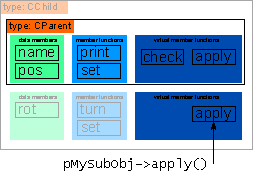
\includegraphics[width=\textwidth]{images/pMySubObj-virtApply}
		
		\column{0.5\textwidth}
		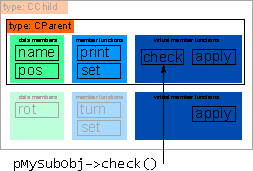
\includegraphics[width=\textwidth]{images/pMySubObj-virtCheck}
	\end{columns}
\end{frame}

\begin{frame}[fragile,b]{Der virtuelle Destruktor}
	Angenommen, ich hätte \verb|pMySubObj = new CChild;| geschrieben. Was macht dann \verb|delete pMySubObj;|?
	
	\pause
	\vspace{1em}
	
	Antwort: Das kommt darauf an, ob der Destruktor von \verb|CParent| virtuell ist!
	\begin{itemize}
		\item Ist der Destruktor \emph{nicht} virtuell, so wird nur \verb|pMySubObj->~CParent()| aufgerufen.
		\item Ist der Destruktor virtuell, so wird zunächst \verb|pMySubObj->~CChild()| und anschließend \verb|pMySubObj->~CParent()| aufgerufen.
	\end{itemize}
	
	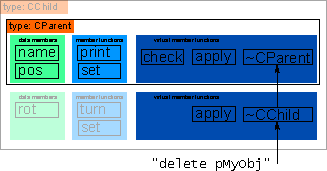
\includegraphics[width=0.5\linewidth]{images/pMySubObj-dtor}
\end{frame}

\begin{frame}[fragile]{Der virtuelle Destruktor, allgemein}
	Der virtuelle Destruktor-Aufruf funktioniert ähnlich wie der Aufruf einer normalen virtuellen Funktion, mit zwei Ausnahmen:
	
	\begin{itemize}
		\item Der Destruktor (dtor) hat in jeder Klasse einen eigenen Namen (\verb|~Classname|).
		\item Es werden \emph{alle} überschriebenen Destruktoren (die der Basisklassen) aufgerufen, und zwar beginnend mit dem dtor im meist abgeleiteten Typ, dann jeweils bei Ende des dtors einer Klasse der dtor der direkten Elterklasse dieser Klasse.
	\end{itemize}
	
	\pause
	\vspace{1em}
	
	Zusätzlich zum dtor-Aufruf wird natürlich noch der Speicher freigegeben. Dabei spielt es keine Rolle, ob der dtor virtuell ist oder nicht.
\end{frame}

\begin{frame}[fragile]{pure virtual member functions}
	Bei einer virtual member function kann die Implementierung komplett weggelassen werden, indem hinter die Funktions-Deklaration ein \verb|= 0;| geschrieben wird. Sie ist dann nur noch eine leere Hülle. Nanu?
	
	\pause
	\vspace{1em}
	
	Die Idee dabei ist: Mit einem \verb|BaseClass*|-Pointer kann man die pure virtual member function ansprechen. Was dann aufgerufen wird, ist eine Überschreibung in einer abgeleiteten Klasse.
\end{frame}

\begin{frame}[fragile,b]{pure virtual member functions: Beispiel}
	Machen wir zum Beispiel die Funktion \verb|apply| in \verb|CParent| zu einer pure virtual member function, also \verb|virtual void apply() = 0;|
	
	\vspace{1em}
	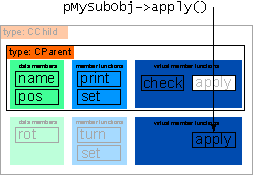
\includegraphics[width=0.5\linewidth]{images/pMySubObj-pureVirtApply}
\end{frame}


\section{Abstrakte Klassen}

\begin{frame}[fragile]{Abstrakte Klassen}
	Es gibt einen Hauptunterschied zwischen:
	\verb|virtual void apply() { }|
	und
	\verb|virtual void apply() = 0;|
	Die erste Variante hat eine \emph{leere} Implementierung (sie tut nichts), während die zweite Variante \emph{keine} Implementierung hat (sie kann nicht selbst aufgerufen werden, sondern nur eine Überschreibung).
	Eine einzige solche pure virtual member function macht eine Klasse zu einer \emph{abstrakten Klasse}.
	
	\pause
	
	\begin{block}{Abstrakte Klassen (Standard, 10.4:1-2)}
		Eine \emph{abstrakte Klasse} ist eine Klasse, die nur als Basisklasse für andere Klassen verwendet werden kann; es können keine Instanzen einer abstrakten Klasse erzeugt werden (nur base class subobjects). Eine Klasse ist eine abstrakte Klasse wenn sie mindestens eine pure virtual member function hat. Beachte: Sie kann diese geerbt haben (wenn noch keine Überschreibung in einer Elterklasse existiert).
	\end{block}
\end{frame}

\begin{frame}[fragile]{Interface}
	Ein abstrakte Klasse, deren member \emph{ausschließlich} pure virtual member functions sind, nennt man auch Interface.
	
	\pause
	\vspace{1em}
	
	Interfaces werden für sehr viele Dinge verwendet und sind neben dem Arbeiten mit Objekten (Instanzen) ein Hauptaspekt im objektorientierten Programmieren. Man definiert mittels Interfaces bspw. die gemeinsame \enquote{Sprache}, mit der zwei voneinander unabhängige Komponenten interagieren können. Die eine Seite nutzt dabei einen Pointer vom Typ \verb|MyInterface*| und die andere Seite \emph{implementiert} das Interface, d.h. hat von eine Klasse, die von \verb|MyInterface| abgeleitet ist und Überschreibungen aller pure virtual member functions enthält. Die letztere Seite erzeugt dann eine Instanz dieser abgeleiteten Klasse und gibt der ersten Seite einen \verb|MyInterface*|-Pointer.
\end{frame}


\section{dynamic\_cast}

\begin{frame}[fragile]{Der Vollständigkeit halber: dynamic\_cast}
	Man kann implizit von einem \verb|CChild*| einen \verb|CParent*| erhalten. Umgekehrt geht das nicht ohne weiteres, denn z.B. ein Pointer auf \verb|myPrObj| kann nicht sinnvollerweise in einen Pointer auf eine \verb|CChild|-Instanz verwandelt werden (z.B.: es fehlt die Information des data members \verb|rot|).
	
	\pause
	\vspace{1em}
	
	Wenn man schreibt \verb|dynamic_cast < CChild* > ( pMySubObj )|, so ist das Resultat dieser expression abhängig vom \emph{dynamic type} von \verb|*pMySubObj|. Verweist \verb|pMySubObj| auf ein base class subobject einer Instanz von \verb|CChild| (z.B. \verb|pMySubObj|), so ist das Ergebnis ein gültiger Pointer auf diese Instanz (auf das »Ding«). Anderenfalls (z.B. \verb|&myPrObj|) ist das Resultat \verb|0|, ein ungültiger Pointer.
\end{frame}
